% Standalone figures for publications
% Compile with: pdflatex -shell-escape standalone_figures.tex
% This generates individual PDF files for each figure

\documentclass[tikz,border=2mm]{standalone}
\usepackage{tikz}
\usetikzlibrary{shapes.geometric, arrows.meta, positioning, fit, calc, backgrounds, patterns, decorations.pathreplacing, shapes.multipart}
\usepackage{pgfplots}
\pgfplotsset{compat=1.17}
\usepackage{amsmath}

% Publication color scheme (print-friendly, grayscale compatible)
\definecolor{blockfill}{RGB}{240,240,240}
\definecolor{emphasisfill}{RGB}{200,200,200}
\definecolor{signalcolor}{RGB}{80,80,80}

\tikzset{
    block/.style={
        rectangle, draw=black, thick, fill=blockfill,
        text centered, minimum height=2em, font=\footnotesize\sffamily
    },
    emphblock/.style={
        block, fill=emphasisfill, font=\footnotesize\sffamily\bfseries
    },
    smallblock/.style={
        block, minimum height=1.5em, font=\scriptsize\sffamily
    },
    dspblock/.style={block, minimum width=2.5cm, minimum height=1.2cm},
    connection/.style={draw=black, thick, -Stealth},
    bus/.style={draw=black, very thick, -Stealth},
    controlsignal/.style={draw=black, dashed, -Stealth},
    label/.style={font=\scriptsize\sffamily},
    statenode/.style={
        circle, draw=black, thick, fill=blockfill,
        text centered, minimum size=1.5cm, font=\scriptsize\sffamily
    }
}

\begin{document}

%==============================================================================
% Figure 1: System Architecture (Publication Version)
%==============================================================================
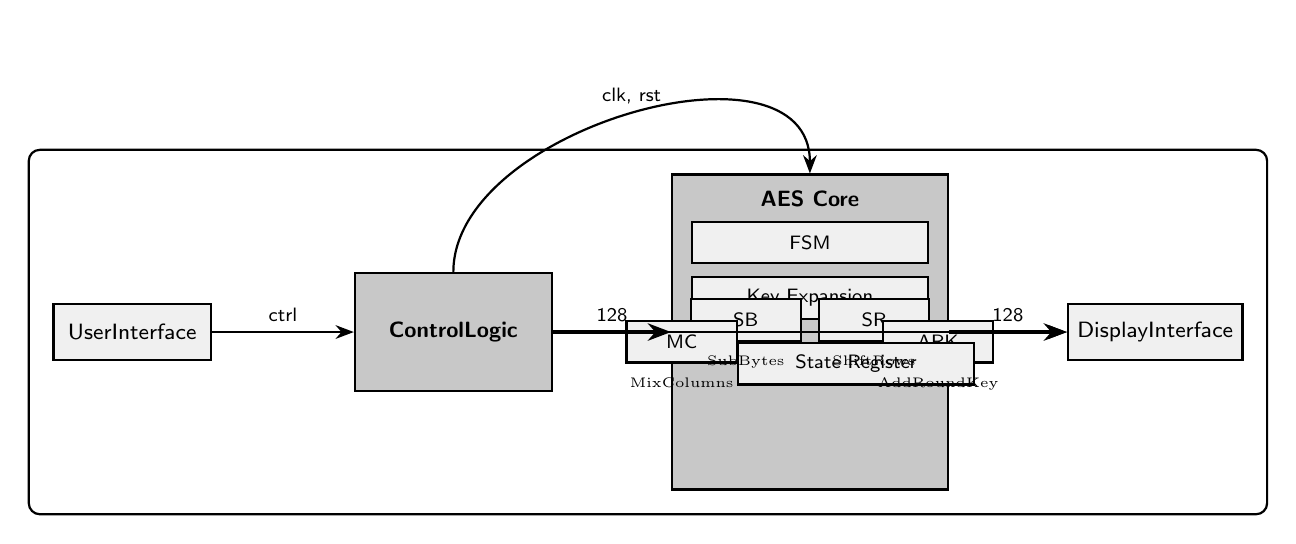
\begin{tikzpicture}[node distance=1.2cm and 1.5cm]

% Input interface
\node[block, minimum width=2cm] (inputs) {User\\Interface};

% Control unit
\node[emphblock, minimum width=2.5cm, minimum height=1.5cm, right=1.8cm of inputs] (control) {Control\\Logic};

% AES Core
\node[emphblock, minimum width=3.5cm, minimum height=4cm, right=1.5cm of control] (core) {};
\node[font=\footnotesize\sffamily\bfseries] at (core.north) [below=0.1cm] {AES Core};

% Core internals
\node[smallblock, minimum width=3cm] (fsm) at (core.north) [below=0.6cm] {FSM};
\node[smallblock, minimum width=3cm] (keyexp) at (fsm.south) [below=0.15cm] {Key Expansion};
\node[smallblock, minimum width=1.4cm] (sub) at (keyexp.south) [below=0.25cm, left=0.1cm] {SB};
\node[smallblock, minimum width=1.4cm] (shift) at (keyexp.south) [below=0.25cm, right=0.1cm] {SR};
\node[smallblock, minimum width=1.4cm] (mix) at (sub.south) [below=0.15cm, left=0.1cm] {MC};
\node[smallblock, minimum width=1.4cm] (ark) at (shift.south) [below=0.15cm, right=0.1cm] {ARK};
\node[smallblock, minimum width=3cm] (state) at (mix.south) [below=0.25cm, right=0.7cm] {State Register};

% Output
\node[block, minimum width=2cm, right=1.5cm of core] (outputs) {Display\\Interface};

% Connections
\draw[connection] (inputs) -- node[label, above] {ctrl} (control);
\draw[bus] (control) -- node[label, above] {128} (core);
\draw[connection] (control) -- (outputs);
\draw[bus] (core) -- node[label, above] {128} (outputs);
\draw[connection] (control) to[out=90, in=90] node[label, above] {clk, rst} (core);

% Annotations
\node[label] at (sub.south) [below=0.05cm, font=\tiny] {SubBytes};
\node[label] at (shift.south) [below=0.05cm, font=\tiny] {ShiftRows};
\node[label] at (mix.south) [below=0.05cm, font=\tiny] {MixColumns};
\node[label] at (ark.south) [below=0.05cm, font=\tiny] {AddRoundKey};

% Bounding box
\begin{scope}[on background layer]
\node[draw=black, thick, rounded corners, fit=(inputs) (control) (core) (outputs), inner sep=0.3cm, label={[font=\small\sffamily]above:FPGA Implementation}] {};
\end{scope}

\end{tikzpicture}
\newpage

%==============================================================================
% Figure 2: AES Core Datapath (Clean Version)
%==============================================================================
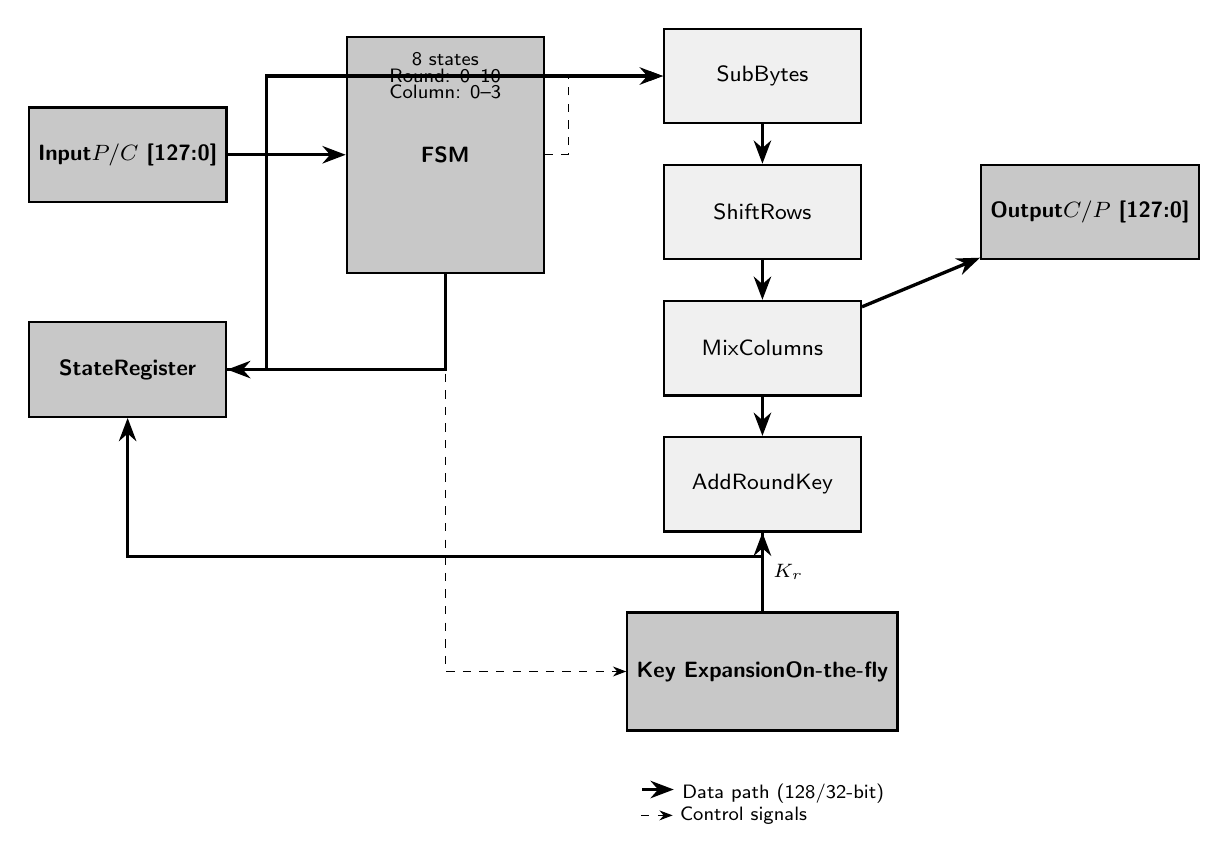
\begin{tikzpicture}[node distance=1cm and 1.5cm]

% Left: Input and state
\node[emphblock, minimum width=2.5cm, minimum height=1.2cm] (input) {Input\\$P/C$ [127:0]};
\node[emphblock, minimum width=2.5cm, minimum height=1.2cm, below=1.5cm of input] (state) {State\\Register};

% Center: FSM
\node[emphblock, minimum width=2.5cm, minimum height=3cm, right=of input] (fsm) {FSM};
\node[label, below=0.1cm of fsm.north] {\scriptsize 8 states};
\node[label, below=0.3cm of fsm.north] {\scriptsize Round: 0--10};
\node[label, below=0.5cm of fsm.north] {\scriptsize Column: 0--3};

% Right: Datapath
\node[dspblock, right=1.5cm of fsm, yshift=1cm] (subbytes) {SubBytes};
\node[dspblock, below=0.5cm of subbytes] (shiftrows) {ShiftRows};
\node[dspblock, below=0.5cm of shiftrows] (mixcols) {MixColumns};
\node[dspblock, below=0.5cm of mixcols] (addrk) {AddRoundKey};

% Bottom: Key expansion
\node[emphblock, minimum width=3cm, minimum height=1.5cm, below=of addrk] (keyexp) {Key Expansion\\On-the-fly};

% Output
\node[emphblock, minimum width=2.5cm, minimum height=1.2cm, right=of shiftrows] (output) {Output\\$C/P$ [127:0]};

% Data connections
\draw[bus] (input) -- (fsm);
\draw[bus] (fsm) |- (state);
\draw[bus] (state.east) -- ++(0.5,0) |- (subbytes);
\draw[bus] (subbytes) -- (shiftrows);
\draw[bus] (shiftrows) -- (mixcols);
\draw[bus] (mixcols) -- (addrk);
\draw[bus] (addrk.south) -- ++(0,-0.3) -| (state);
\draw[bus] (mixcols) -- (output);

% Key connection
\draw[bus] (keyexp) -- node[label, right] {$K_r$} (addrk);

% Control
\draw[controlsignal] (fsm) |- (keyexp);
\draw[controlsignal] (fsm.east) -- ++(0.3,0) |- (subbytes);

% Legend
\node[label, below=0.5cm of keyexp, align=left] {
\tikz{\draw[bus] (0,0) -- (0.4,0);} Data path (128/32-bit)\\
\tikz{\draw[controlsignal] (0,0) -- (0.4,0);} Control signals
};

\end{tikzpicture}
\newpage

%==============================================================================
% Figure 3: State Machine (Simplified)
%==============================================================================
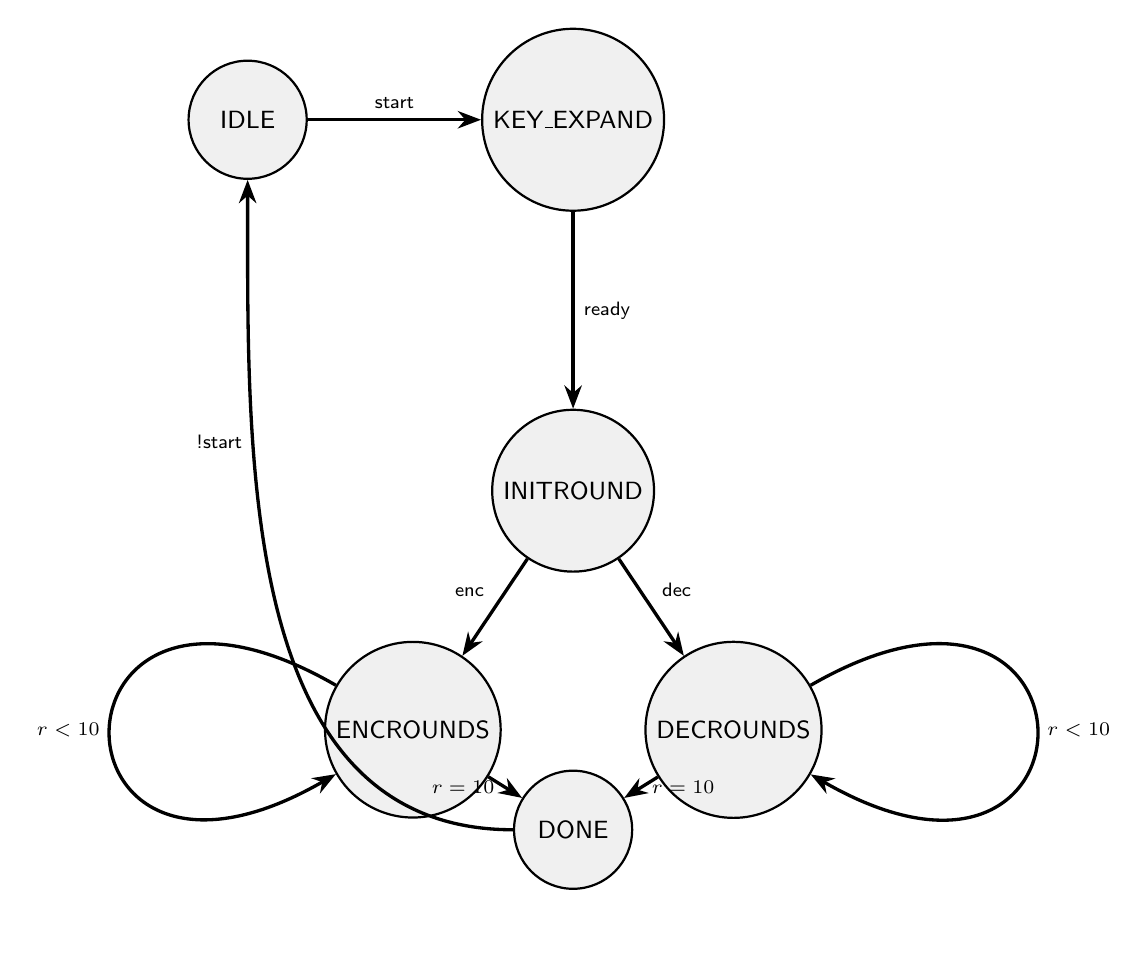
\begin{tikzpicture}[node distance=2.5cm]

% States
\node[statenode, font=\small\sffamily] (idle) {IDLE};
\node[statenode, font=\small\sffamily, right=2.2cm of idle] (keyexp) {KEY\_\\EXPAND};
\node[statenode, font=\small\sffamily, below=of keyexp] (init) {INIT\\ROUND};
\node[statenode, font=\small\sffamily, below left=1.5cm and 0.5cm of init] (encrypt) {ENC\\ROUNDS};
\node[statenode, font=\small\sffamily, below right=1.5cm and 0.5cm of init] (decrypt) {DEC\\ROUNDS};
\node[statenode, font=\small\sffamily, below=2.5cm of init] (done) {DONE};

% Transitions
\draw[connection, very thick] (idle) -- node[label, above] {start} (keyexp);
\draw[connection, very thick] (keyexp) -- node[label, right] {ready} (init);
\draw[connection, very thick] (init) -- node[label, above left] {enc} (encrypt);
\draw[connection, very thick] (init) -- node[label, above right] {dec} (decrypt);
\draw[connection, very thick] (encrypt) -- node[label, left] {$r=10$} (done);
\draw[connection, very thick] (decrypt) -- node[label, right] {$r=10$} (done);
\draw[connection, very thick] (done) to[out=180, in=270] node[label, left, pos=0.7] {!start} (idle);

% Self loops for rounds
\draw[connection, very thick] (encrypt) to[out=150, in=210, looseness=10] node[label, left] {$r<10$} (encrypt);
\draw[connection, very thick] (decrypt) to[out=30, in=-30, looseness=10] node[label, right] {$r<10$} (decrypt);

\end{tikzpicture}
\newpage

%==============================================================================
% Figure 4: Column-Wise Processing
%==============================================================================
\begin{tikzpicture}[node distance=1.2cm]

% State matrix
\node[label, font=\footnotesize\sffamily\bfseries] (title) {128-bit State Matrix};

\node[below=0.3cm of title] (matrix) {
\begin{tikzpicture}[scale=0.8]
    % 4x4 grid
    \draw[thick] (0,0) grid (4,4);

    % Column highlighting
    \draw[red, very thick] (0,0) rectangle (1,4);
    \node[red, font=\tiny] at (0.5,-0.3) {Col 0};

    \draw[blue, very thick] (1,0) rectangle (2,4);
    \node[blue, font=\tiny] at (1.5,-0.3) {Col 1};

    \draw[green!60!black, very thick] (2,0) rectangle (3,4);
    \node[green!60!black, font=\tiny] at (2.5,-0.3) {Col 2};

    \draw[orange, very thick] (3,0) rectangle (4,4);
    \node[orange, font=\tiny] at (3.5,-0.3) {Col 3};

    % Labels
    \node[font=\tiny] at (0.5,3.5) {$s_{0,0}$};
    \node[font=\tiny] at (0.5,2.5) {$s_{1,0}$};
    \node[font=\tiny] at (0.5,1.5) {$s_{2,0}$};
    \node[font=\tiny] at (0.5,0.5) {$s_{3,0}$};

    \node[font=\tiny] at (3.5,3.5) {$s_{0,3}$};
    \node at (2,2) {$\cdots$};
\end{tikzpicture}
};

% Processing sequence
\node[emphblock, right=2cm of matrix, minimum width=2.5cm] (proc) {32-bit\\Processing\\Unit};

\node[smallblock, above=0.3cm of proc] (op1) {SubBytes};
\node[smallblock, below=0.1cm of proc] (op2) {MixColumns};
\node[smallblock, below=0.1cm of op2] (op3) {AddRoundKey};

% Timing
\node[below=1.2cm of proc, font=\footnotesize\sffamily\bfseries] (timing) {Sequential Processing};

\node[below=0.2cm of timing] (timeline) {
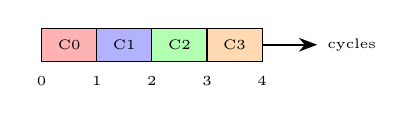
\begin{tikzpicture}[scale=0.7]
    % Timeline
    \draw[thick, -Stealth] (0,0) -- (5,0) node[right, font=\tiny] {cycles};

    % Time blocks
    \draw[fill=red!30] (0,-0.3) rectangle (1,0.3) node[midway, font=\tiny] {C0};
    \draw[fill=blue!30] (1,-0.3) rectangle (2,0.3) node[midway, font=\tiny] {C1};
    \draw[fill=green!30] (2,-0.3) rectangle (3,0.3) node[midway, font=\tiny] {C2};
    \draw[fill=orange!30] (3,-0.3) rectangle (4,0.3) node[midway, font=\tiny] {C3};

    % Tick marks
    \foreach \x in {0,1,2,3,4} {
        \draw (\x,0.1) -- (\x,-0.1);
        \node[below, font=\tiny] at (\x,-0.4) {\x};
    }
\end{tikzpicture}
};

% Arrows
\draw[bus] (matrix) -- node[label, above] {32 bits} (proc);

% Annotation
\node[below=0.5cm of timeline, align=center, font=\scriptsize] {
4 cycles per operation\\
Resource savings: 75\%
};

\end{tikzpicture}
\newpage

%==============================================================================
% Figure 5: Key Expansion Diagram
%==============================================================================
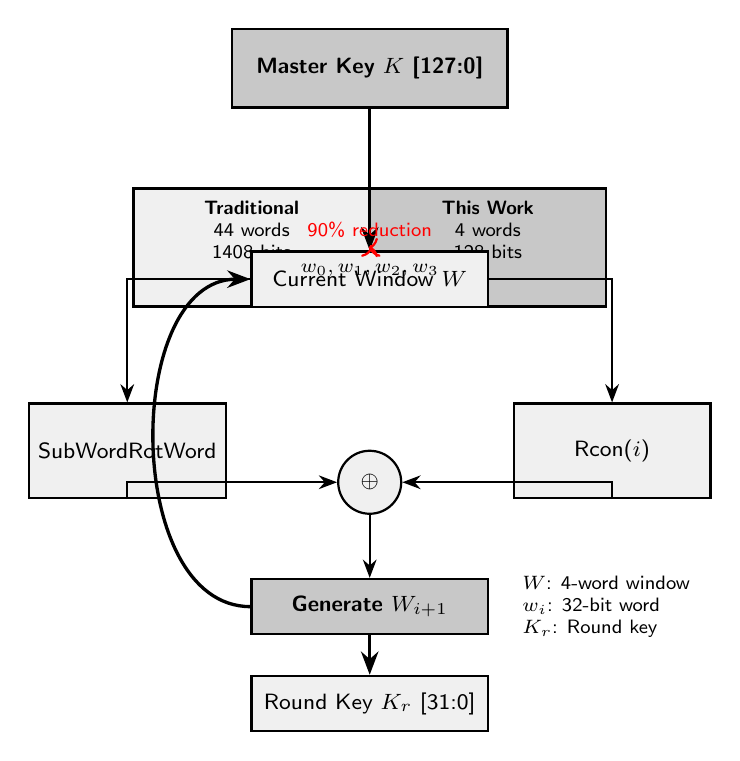
\begin{tikzpicture}[node distance=1cm and 1.2cm]

% Master key input
\node[emphblock, minimum width=3.5cm, minimum height=1cm] (master) {Master Key $K$ [127:0]};

% Storage comparison
\node[block, minimum width=3cm, minimum height=1.5cm, below=of master, xshift=-1.5cm] (traditional) {};
\node[label, below=0.05cm of traditional.north, align=center] {\textbf{Traditional}\\44 words\\1408 bits};

\node[emphblock, minimum width=3cm, minimum height=1.5cm, below=of master, xshift=1.5cm] (otf) {};
\node[label, below=0.05cm of otf.north, align=center] {\textbf{This Work}\\4 words\\128 bits};

% Current window
\node[block, minimum width=3cm, below=1.8cm of master] (window) {Current Window $W$};
\node[label, below=0.05cm of window.north] {$w_0, w_1, w_2, w_3$};

% Processing blocks
\node[dspblock, below left=1.2cm and 0.3cm of window] (subword) {SubWord\\RotWord};
\node[dspblock, below right=1.2cm and 0.3cm of window] (rcon) {Rcon($i$)};

% XOR
\node[block, circle, minimum size=0.8cm, below=1.8cm of window] (xor) {$\oplus$};

% Generation
\node[emphblock, minimum width=3cm, below=0.8cm of xor] (gen) {Generate $W_{i+1}$};

% Output
\node[block, minimum width=3cm, below=0.5cm of gen] (output) {Round Key $K_r$ [31:0]};

% Connections
\draw[bus] (master) -- (window);
\draw[connection] (window) -| (subword);
\draw[connection] (window) -| (rcon);
\draw[connection] (subword) |- (xor);
\draw[connection] (rcon) |- (xor);
\draw[connection] (xor) -- (gen);
\draw[bus] (gen) to[out=180, in=180] (window);
\draw[bus] (gen) -- (output);

% Annotation - storage savings
\draw[<->, thick, red] (traditional.east) -- node[label, above, red] {90\% reduction} (otf.west);

% Legend
\node[label, right=0.3cm of gen, align=left] {
$W$: 4-word window\\
$w_i$: 32-bit word\\
$K_r$: Round key
};

\end{tikzpicture}
\newpage

%==============================================================================
% Figure 6: Performance Chart
%==============================================================================
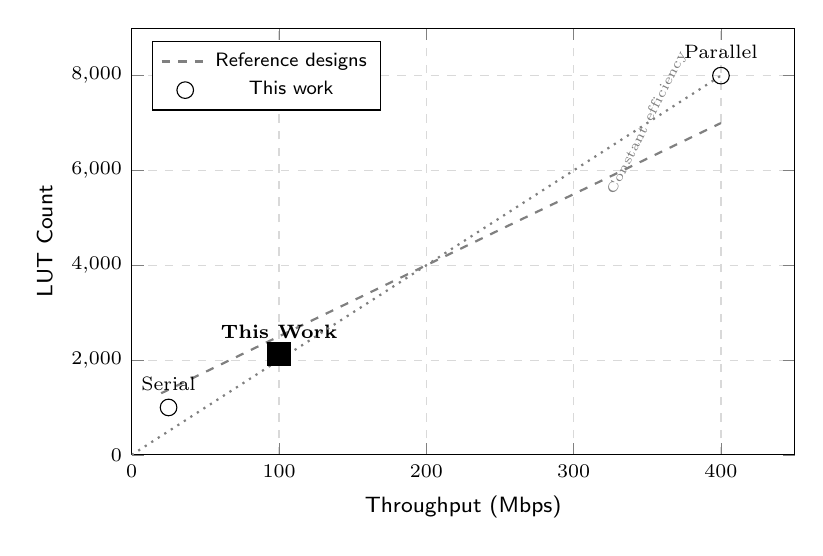
\begin{tikzpicture}
\begin{axis}[
    xlabel={Throughput (Mbps)},
    ylabel={LUT Count},
    xmin=0, xmax=450,
    ymin=0, ymax=9000,
    width=10cm,
    height=7cm,
    grid=major,
    grid style={dashed, gray!30},
    legend pos=north west,
    xlabel style={font=\footnotesize\sffamily},
    ylabel style={font=\footnotesize\sffamily},
    tick label style={font=\scriptsize\sffamily},
    legend style={font=\scriptsize\sffamily}
]

% Area-throughput curve (approximate)
\addplot[domain=20:400, samples=50, thick, gray, dashed] {1000 + 15*x};

% Data points
\addplot[only marks, mark=o, mark size=3pt, color=black] coordinates {
    (25, 1000)
    (400, 8000)
};

% This work
\addplot[only marks, mark=square*, mark size=4pt, color=black, thick] coordinates {
    (100, 2132)
};

% Labels
\node[font=\scriptsize, align=center] at (axis cs:25,1500) {Serial};
\node[font=\scriptsize, align=center] at (axis cs:100,2600) {\textbf{This Work}};
\node[font=\scriptsize, align=center] at (axis cs:400,8500) {Parallel};

% Efficiency line
\draw[thick, gray, dotted] (axis cs:0,0) -- (axis cs:400,8000);
\node[font=\tiny, gray] at (axis cs:350,7000) [rotate=63] {Constant efficiency};

\legend{Reference designs, This work}

\end{axis}
\end{tikzpicture}
\newpage

%==============================================================================
% Figure 7: Resource Bar Chart
%==============================================================================
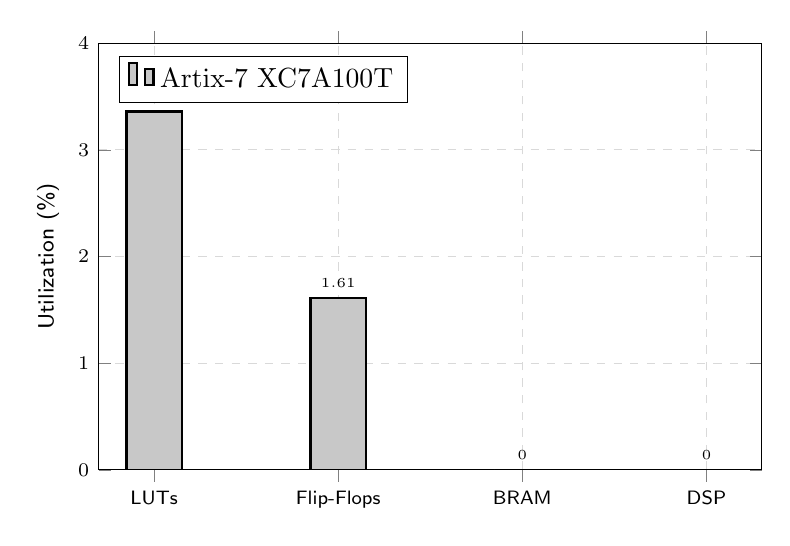
\begin{tikzpicture}
\begin{axis}[
    ybar,
    bar width=20pt,
    ylabel={Utilization (\%)},
    symbolic x coords={LUTs, Flip-Flops, BRAM, DSP},
    xtick=data,
    ymin=0, ymax=4,
    width=10cm,
    height=7cm,
    legend pos=north west,
    grid=major,
    grid style={dashed, gray!30},
    ylabel style={font=\footnotesize\sffamily},
    xlabel style={font=\footnotesize\sffamily},
    tick label style={font=\scriptsize\sffamily},
    nodes near coords,
    nodes near coords style={font=\tiny},
    every node near coord/.append style={rotate=0, anchor=south}
]

\addplot[fill=emphasisfill, draw=black, thick] coordinates {
    (LUTs, 3.36)
    (Flip-Flops, 1.61)
    (BRAM, 0)
    (DSP, 0)
};

\legend{Artix-7 XC7A100T}

\end{axis}
\end{tikzpicture}

\end{document}
